\documentclass[../TDE1-E2.tex]{subfiles}%

\begin{document}
\section[s]"2"{Pont de Wheatstone}

\QR{%
  \noindent
\begin{minipage}{0.65\linewidth}
  En électronique, on réalise régulièrement des ponts de mesure pour mesurer
  indirectement une résistance. On dispose d'un circuit comprenant un
  générateur de tension qui alimente un pont de Wheatstone composé des
  résistances $R_1$ et $R_2$. La résistance $R_i$ est inconnue, et la
  résistance $R$ est variable (il s'agit d'un potentiomètre). On fait évoluer
  $R$ jusqu'à ce que le voltmètre indique une tension nulle. Le pont est alors
  équilibré.
  \bigbreak
  À l'aide des lois de Kirchhoff, déterminer l'expression de la valeur de
  $R_i$ en fonction des valeurs des autres résistances lorsque le pont est
  équilibré.
\end{minipage}
\hfill
\begin{minipage}{0.35\linewidth}
  \begin{center}
    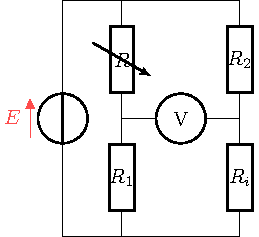
\includegraphics[width=\linewidth]{wheatstone-plain}
  \end{center}
\end{minipage}
}{%
\vspace{-15pt}
\begin{tcbraster}[raster columns=6, raster equal height=rows]
    \begin{tcn}[raster multicolumn=2](data){Schéma}
        \begin{center}
            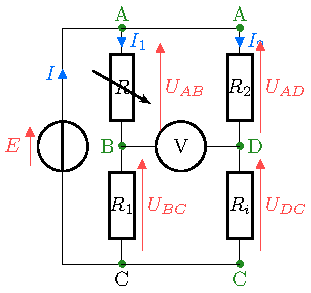
\includegraphics{wheatstone}
        \end{center}
    \end{tcn}
    \begin{tcolorbox}[blankest, raster multicolumn=1, space to=\myspace]
        \begin{tcbraster}[raster columns=1]
            \begin{tcn}[add to natural height=\myspace](ques)""{Résultat}

                \fontsize{10pt}{12pt}\selectfont On cherche $R_i$, ou $U_{DC}$
                quand «~le pont est équilibré~».

            \end{tcn}
            \begin{tcn}(tool)""{Outil}

                \fontsize{10pt}{12pt}\selectfont D'après l'énoncé, le pont est
                équilibré quand $V = 0$, soit quand $V_B = V_D$.

            \end{tcn}
        \end{tcbraster}
    \end{tcolorbox}
    \begin{tcn}[raster multicolumn=3](appl)'r'{Application}
        Si le pont est équilibré, alors $U_{AB} = U_{AD}$ et $U_{BC} = U_{DC}$.
        Or, avec le pont diviseur de tension, on a à la fois
        \begin{align*}
            U_{BC} & = E \frac{R_1}{R_1+R}\\
            U_{DC} & = E \frac{R_i}{R_i+R_2}
        \end{align*}
        Donc
        \begin{align*}
            U_{BC} &= U_{DC}\\
            \Leftrightarrow \cancel{E} \frac{R_1}{R_1+R}
                   & = \cancel{E} \frac{R_i}{R_i+R_2}\\
            \Leftrightarrow R_1(\cancel{R_i}+R_2) & = R_i(\cancel{R_1}+R)\\
            \Leftrightarrow \Aboxed{R_i & = \frac{R_1R_2}{R}}
        \end{align*}
    \end{tcn}
\end{tcbraster}
}%

\end{document}
